%% Public domain image from
%% http://www.public-domain-image.com/objects/computer-chips/slides/six-computers-chips-circuits.html
\renewcommand\chapterillustration{Math_quaternion/chapterImage}



\chapter{사원수와 회전}
\index{사원수}
\index{quaternion}

사원수(quaternion)는 스칼라(scalar) 값과 3차원 벡터를 묶어 구성한 복소수(complex number)이다.
3차원 벡터 $\mathbf v = (a, b, c)$를 각각의 축 방향 단위 벡터인 기저 $\mathbf i, \mathbf  j, \mathbf k$로 표현하면 $a{\mathbf i} + b {\mathbf j} + c {\mathbf k}$이다.
사원수는 여기에 스칼라 값 $d$가 추가된 $d + a{\mathbf i} + b {\mathbf j} + c {\mathbf k}$이다.
기저를 제외하고 표현하면 $(d, (a, b, c))$와 같이 표현된다. 벡터 기호로 표현하면 이는 $(d, \mathbf v)$가 된다.
스칼라 값은 기저가 실수의 단위 값인 1이라고 이해하면 사원수는 $1, \mathbf i, \mathbf  j, \mathbf k$를 기저로 하는 벡터라고 할 수도 있다.
이 사원수는 로보틱스와 컴퓨터 그래픽스 분야에서 회전을 다루는 데에 빈번히 이용된다. 이 장에서는 이 사원수와 회전의 관계에 대해 이해해 볼 것이다.

\section{사원수의 연산}
\index{사원수!연산}
\index{quaternion!operations}

사원수와 회전의 관계를 살펴보기 전에 사원수의 연산 방법에 대해서 먼저 살펴 보자.
4원수는 단순한 4차원 벡터와 유사한 성격을 갖는다.
따라서 연산 역시 벡터의 연산과 큰 차이가 없다.

\subsection{사원수의 덧셈과 뺄셈}
우선 사원수의 덧셈을 살펴 보자. 벡터의 덧셈은 대응되는 성분별로 더하면 된다.
두 개의 사원수 $\hat{p}$와 $\hat{q}$가 각각 $(s_p, \mathbf v_p)$와 $(s_q, \mathbf v_q)$라고 하자.
두 사원수의 합은 다음과 같다.

$$\hat{p} + \hat{q} = (s_p + s_q , \mathbf v_p + \mathbf v_q )$$

만약 두 사원수를 $\hat{p} = (a_p, b_p, c_p, d_p)$와 $\hat{q} = (a_q, b_q, c_q, d_q)$로 표현한다면 두 사원수의 합은 
간단히 다음과 같이 표현된다.

$$\hat{p} + \hat{q} = (a_p + a_q, b_p + b_q , c_p + c_q , d_p + d_q)$$

뺄셈 역시 덧셈과 같이 성분 별로 이루어진다.

$$\hat{p} - \hat{q} = (a_p - a_q, b_p - b_q , c_p - c_q , d_p - d_q)$$

스칼라와 벡터로 나누어 표현하면 다음과 같다.

$$\hat{p} = (s_p, \mathbf v_p), \hat{q} = (s_q, \mathbf v_q)$$
$$\hat{p} + \hat{q} = (s_p - s_q , \mathbf v_p - \mathbf v_q )$$

\subsection{사원수의 곱셈}
\index{사원수!곱셈}
\index{quaternion!multiplication}

사원수와 어떤 스칼라 $\lambda$를 곱하는 것은 매우 간단하다. 사원수의 모든 성분에 이 스칼라 값을 곱하면 된다.
따라서 사원수의 스칼라 곱은 다음과 같이 표현할 수 있다.

$$\lambda \hat{p} = (\lambda s_p , \lambda \mathbf v_p) = (\lambda a_p, \lambda b_p, \lambda c_p, \lambda d_p)$$

이제 두 사원수 $\hat{p}$와 $\hat{q}$를 곱하려면 어떻게 해야 할까?
앞서 말한 바와 같이 사원수는 각각의 기저를 서로 다른 허수 $\mathbf i, \mathbf j, \mathbf k$로 보고,
벡터 부분의 각 성분은 이 허수에 곱해진 값이고, 스칼라 부분을 더해서 얻는 복소수로 볼 수 있다.
이때 $\mathbf i^2 = \mathbf j^2 = \mathbf k^2 = -1$이고, $\mathbf {ij} = \mathbf k$, 
$\mathbf {jk} = \mathbf i$, $\mathbf {ki} = \mathbf j$의 관계를 가진다. 그리고 
$\mathbf {ji} = -\mathbf k$, $\mathbf {kj} = -\mathbf i$, $\mathbf {ik} = -\mathbf j$이다.

따라서 $\hat{p} \hat{q}$는 다음과 같이 표현할 수 있다.

\begin{eqnarray}
\hat{p} & = & d_p + a_p{\mathbf i} + b_p{\mathbf j} + c_p{\mathbf k} \\ \nonumber
\hat{q} & = & d_q + a_q{\mathbf i} + b_q{\mathbf j} + c_q{\mathbf k} \\ \nonumber
\hat{p}\hat{q} &=& (d_p + a_p{\mathbf i} + b_p{\mathbf j} + c_p{\mathbf k} )(d_q + a_q{\mathbf i} + b_q{\mathbf j} + c_q{\mathbf k})
\end{eqnarray}

조금 수고스럽기는 하지만, 이를 푸는 것은 매운 단순한 계산이다. 결과는 다음과 같다.

\begin{eqnarray}
\hat{p}\hat{q} = &
d_p d_q + d_p + d_p a_q{\mathbf i} + d_p b_q{\mathbf j} + d_p c_q{\mathbf k} + \\ \nonumber
& a_p {\mathbf i} d_q + a_p {\mathbf i}  a_q{\mathbf i} + a_p {\mathbf i} b_q{\mathbf j} + a_p {\mathbf i}  c_q{\mathbf k} + \\ \nonumber
& b_p {\mathbf j} d_q + b_p {\mathbf j} a_q{\mathbf i} + b_p {\mathbf j} b_q{\mathbf j} + b_p {\mathbf j} c_q{\mathbf k} + \\ \nonumber
& c_p {\mathbf k} d_q + c_p {\mathbf k} a_q{\mathbf i} + c_p {\mathbf k} b_q{\mathbf j} + c_p {\mathbf k} c_q{\mathbf k} 
\end{eqnarray}

이를 조금 정리하면 다음과 같은 꼴이 된다.

\begin{eqnarray}
\hat{p}\hat{q} = &
d_p d_q + d_p a_q{\mathbf i} + d_p b_q{\mathbf j} + d_p c_q{\mathbf k} + \\ \nonumber
& a_p d_q{\mathbf i}  + a_p a_q {\mathbf i}^2 + a_p b_q{\mathbf i} {\mathbf j} + a_p c_q {\mathbf i}  {\mathbf k} + \\ \nonumber
& b_p d_q {\mathbf j} + b_p a_q {\mathbf j} {\mathbf i} + b_p b_q{\mathbf j}^2 + b_p c_q {\mathbf j} {\mathbf k} + \\ \nonumber
& c_p d_q{\mathbf k}  + c_p a_q{\mathbf k} {\mathbf i} + c_p b_q{\mathbf k} {\mathbf j} + c_p c_q {\mathbf k}^2
\end{eqnarray}

허수가 나타나는 부분을 정리하면 다음과 같다.

\begin{eqnarray}
\hat{p}\hat{q} = &
d_p d_q + d_p a_q{\mathbf i} + d_p b_q{\mathbf j} + d_p c_q{\mathbf k} + \\ \nonumber
& a_p d_q{\mathbf i}  - a_p a_q + a_p b_q{\mathbf k} - a_p c_q {\mathbf j} + \\ \nonumber
& b_p d_q {\mathbf j} - b_p a_q {\mathbf k} - b_p b_q + b_p c_q {\mathbf i} + \\ \nonumber
& c_p d_q {\mathbf k}  + c_p a_q{\mathbf j} - c_p b_q{\mathbf i} - c_p c_q 
\end{eqnarray}

허수별로 정리하면 다음과 같다.

\begin{eqnarray}
\hat{p}\hat{q} = & d_p d_q  - a_p a_q - b_p b_q - c_p c_q  \\ \nonumber
&+ d_p a_q{\mathbf i} + a_p d_q{\mathbf i} + (b_p c_q - c_p b_q ) {\mathbf i}  \\ \nonumber
&+ d_p b_q{\mathbf j} + b_p d_q {\mathbf j} + (c_p a_q - a_p c_q) {\mathbf j} \\ \nonumber
&+ d_p c_q{\mathbf k} + c_p d_q {\mathbf k} + (a_p b_q - b_p a_q) {\mathbf k}
\end{eqnarray}


이 계산의 의미는 다음과 같다.

\begin{eqnarray}
\hat{p}\hat{q} = & d_p d_q  - (a_p a_q + b_p b_q + c_p c_q)  \\ \nonumber
&+ d_p ( a_q{\mathbf i} + b_q {\mathbf j} + c_q {\mathbf k}) \\ \nonumber
&+ d_q ( a_p{\mathbf i} + b_p {\mathbf j} + c_p {\mathbf k}) \\ \nonumber
&+ (b_p c_q - c_p b_q ) {\mathbf i}  + (c_p a_q - a_p c_q) {\mathbf j} + (a_p b_q - b_p a_q) {\mathbf k}
\end{eqnarray}

이를 벡터의 내적과 외적을 이용하여 설명하면 다음과 같음을 쉽게 알 수 있다.

\begin{eqnarray}
\hat{p}\hat{q} = & d_p d_q  - (\mathbf v_p \cdot \mathbf v_q)  \\ \nonumber
&+ d_p \mathbf v_q + d_q \mathbf v_p + \mathbf v_p \times \mathbf v_q 
\end{eqnarray}

사원수를 스칼라 값과 벡터 표현인 $(d, \mathbf v)$로 표현하면 다음과 같은 방식으로 곱해짐을 알 수 있다.
\begin{eqnarray}
\hat{p}\hat{q} & = & (d_p, \mathbf v_p) (d_q , \mathbf v_q) \\ \nonumber
& =  & ( d_p d_q  - \mathbf v_p \cdot \mathbf v_q , d_p \mathbf v_q + d_q \mathbf v_p + \mathbf v_p \times \mathbf v_q ) 
\end{eqnarray}


이것의 의미를 설명하자면, 스칼라와 벡터로 이루어진 사원수 둘을 곱하면
새로운 사원수가 나타난다는 것이다. 이렇게 얻은 사원수의 스칼라는 곱해진 두 사원수가 가진 스칼라 값의 곱에서
두 사원수가 가진 벡터를 내적한 결과를 빼준 것이다. 내적 결과가 스칼라이므로 이 값은 어려움 없이 구할 수 있다.
결과 사원수의 벡터 부분은 각 사원수가 가진 스칼라 값을 상대편의 벡터 부분에 곱한 결과 두 개를 더하고,
두 사원수가 가진 벡터를 서로 외적하여 얻는 벡터를 추가로 더하여 얻는다는 것이다.


\subsection{사원수 연산 규칙}
\index{사원수!연산 규칙}

사원수는 다음과 같은 연산 규칙을 갖는다.

$$\hat{p} + \hat{q} = \hat{q} + \hat{p}$$
$$(\hat{p} + \hat{q}) + \hat{r} = \hat{p} + (\hat{q} + \hat{r} )$$
$$\lambda \hat p = \hat p \lambda$$
$$- \lambda \hat p = \lambda ( - \hat p)$$
$$\hat p \hat q \neq \hat q \hat p$$

모든 사원수는 그 짝이 되는 켤레 사원수(공액 사원수, conjugate)를 가진다. 
어떤 사원수 $\hat p = (d_p, \mathbf v_p)$의 켤레 사원수를 $\hat p^*$라고 하면 이 사원수는 $(d_p, - \mathbf v_p)$의 값을 가진다.

$$\hat p = (d_p ,  \mathbf v_p) \Rightarrow \hat p^* = (d_p , -\mathbf v_p)$$

사원수의 크기는 벡터의 크기와 같은 방식으로 구한다.
어떤 사원수 $\hat q = (d_q, \mathbf v(a_q, b_q, c_q))$의 크기를 $|\hat q|$로 표현하면, 이 값은 다음과 같다.

\begin{eqnarray}
|\hat q| & = &\sqrt{d_q  d_q + a_q a_q + b_q b_q + c_q c_q} \\ \nonumber
& = & \sqrt{d_q^2 + a_q^2 + b_q^2 + c_q^2} \\ \nonumber
& = & \sqrt{d_q^2 + \mathbf v^{\rm T} \mathbf v} \\ \nonumber
& = & \sqrt{d_q^2 + \mathbf v \cdot \mathbf v} \\ \nonumber
& = & \sqrt{\hat q \hat q^*}
\end{eqnarray}

사원수의 항등원 $\hat i$는 $(1,0,0,0)$이다.
사원수 $\hat q$의 역원 $\hat q^{-1}$은 $\hat q^* / |\hat q|$이다.
그 정의에 의해 다음이 성립한다.

$$\hat q \hat i = \hat i \hat q = \hat q$$
$$\hat q \hat q^{-1} = \hat q^{-1} \hat q = \hat q \hat q^* / |q| = \hat i$$

위 식에서도 쉽게 유추할 수 있고, 간단히 계산을 해 보아도 알 수 있듯이 켤레 사원수의 크기는 서로 동일하다.

$$|\hat q| = |\hat q^*|$$

그리고 다음과 같은 연산 규칙도 중요하다.

$$(\hat q + \hat r)^* = \hat q^* + \hat r^*$$
$$(\hat q \hat r)^* = \hat r^* \hat q^*$$

\section{사원수와 회전의 관계}
\index{사원수!회전과의 관계}
\index{quaternion!rotation and quaternion}

우리는 앞서 회전을 행렬로 표현하는 방법에 대해 다룬 적이 있다.
그런데 회전은 지금까지 다룬 사원수를 이용하여 표현할 수도 있다.
사실 컴퓨터 그래픽스를 다루는 이 책에서 사원수를 다루는 이유는 사원수가 회전 변환을 표현하는 데에 유용하기 때문이다.
3차원 공간의 좌표는 3차원 벡터로 표현할 수 있기 때문에 스칼라 값이 0이고 벡터 부분만 가진 사원수로 표현할 수 있다.
그러면 어떤 좌표 ${\mathbf p}(x,y,z)$는 사원수 표현으로는 $\hat p=(0, (x,y,z))=(0, \mathbf p)$로 표현할 수 있다.
여기에다가 다음과 같은 사원수 $\hat q$를 곱하면 어떻게 되는지 살펴보자.

\begin{eqnarray}
\hat p = (0, \mathbf p) \\ \nonumber
\hat q = (\cos \theta, \sin \theta \mathbf u), |\mathbf u| = 1, |\hat q| = 1
\label{eq:quaternionsToBeMultiplied}
\end{eqnarray}

여기에 사용된 벡터 $\mathbf u$는 단위벡터이다. 이는 곧 $\mathbf u$가 어떤 방향이나 축(axis)를 표현한다는 것이다.
앞에서 살펴본 곱셈 연산법을 통해 이 둘의 곱이 다음과 같음을 쉽게 알 수 있다.

\begin{eqnarray}
\hat p' = (d_{p'}, \mathbf p') \\ \nonumber
\hat p' = \hat q \hat p =  (-\sin \theta \mathbf u \cdot \mathbf p , \cos \theta \mathbf p + \sin \theta \mathbf u \times \mathbf p)
\label{eq:quaternionOrtho}
\end{eqnarray}

\subsection{곱해진 사원수의 벡터 부분들이 직교인 특수한 경우}

식 \ref{eq:quaternionsToBeMultiplied}의 두 사원수를 이용하여 
이러한 사원수의 곱이 회전과 어떠한 관련이 있는지에 대한 기본적인 이해를 얻기 위해 
$\mathbf p$와 $\mathbf u$가 서로 직교하는 경우를 가정해 보자.
그림 \ref{fig:quaternion:quaternionOrtho}가 이러한 경우를 시각적으로 보이고 있다.
이 그림을 통해 사원수의 곱과 회전의 관계를 살펴 보자.

어떤 단위 벡터 $\mathbf u$와 임의의 벡터 $\mathbf p$는 서로 직교하다고 가정했다. 이 두 벡터를 외적한 $\mathbf u \times \mathbf p$는
그림에서 $\mathbf p$를 $\mathbf u$ 축을 중심으로 90도 회전한 것과 같다. 따라서 $\mathbf u$, $\mathbf p$, $\mathbf u \times \mathbf p$는
직교 좌표계의 세 축 위에 놓일 수 있다. 좌표축은 단위 벡터로 표현되어야 하기 때문에 다음과 같은 세 벡터가 직교 좌표축을 이룬다.

$$\mathbf u, ~~~\frac{\mathbf p}{ |\mathbf p| }, ~~~\frac{\mathbf u \times \mathbf p}{|\mathbf p|}$$

이제 $\mathbf p$를 $\mathbf u$를 중심축으로 $\theta$만큼 회전시킨 점 $\mathbf p'$을 살펴 보자.
이 점은 $\frac{\mathbf p}{ |\mathbf p| }$축 방향으로의 길이 $\alpha$와 $\frac{\mathbf u \times \mathbf p}{|\mathbf p|}$축 방향으로의 
길이 $\beta$를 안다면 $\alpha \frac{\mathbf p}{ |\mathbf p| } + \beta \frac{\mathbf u \times \mathbf p}{|\mathbf p|}$로 표현할 수 있다.
그림에서 볼 수 있는 바와 같이 삼각함수의 성질을 고려하면 $\alpha = |\mathbf p| \cos \theta$임을 쉽게 알 수 있고,
$\beta = |\mathbf p| \sin \theta$임도 쉽게 알 수 있다.
따라서 회전된 좌표 $\mathbf p'$는 $ \cos \theta \mathbf p + \sin \theta \mathbf u \times \mathbf p$임을 알 수 있다.
이것은 식 \ref{eq:quaternionOrtho}에 나타난 두 사원수의 곱으로 얻은 사원수의 벡터 부분과 동일하다. 그리고 이 식의 스칼라 부분은 
이 예에서 가정한 $\mathbf u  \perp \mathbf p$의 경우라면 0이 되므로, 사원수의 곱이 회전과 매우 밀접한 관계를 갖고 있음을 확인할 수 있다.



\begin{figure}[h!]
  \centering
    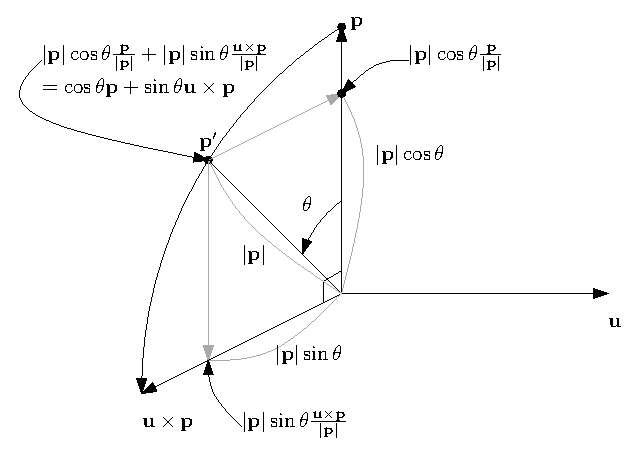
\includegraphics[width=12cm]{Math_quaternion/quaternionOrtho.eps}
    \caption{단위 벡터 $\mathbf u$와 수직인 $\mathbf p$에 대해 사원수 $(\cos \theta, \sin \theta \mathbf u)$와 $(0, \mathbf p)$를 곱한 결과와 회전의 관계}
    \label{fig:quaternion:quaternionOrtho}
\end{figure}


\subsection{일반적 경우의 사원수 곱과 회전의 관계}

앞에서 살펴본 내용은 사원수의 곱이 회전과 관련되어 있다는 직관을 제공하기는 하지만 일반적인 경우가 아니다.
$\mathbf p$와 $\mathbf u$가 서로 직교한다는 가정부터 일반적인 경우가 아니다.
일반적인 경우에는 두 벡터가 직교하지 않기 때문에 0이 아닌 스칼라 부분 $-\sin \theta \mathbf u \cdot \mathbf p$를 가지게 된다.
내적의 특성에 따라 이 $\mathbf p$와 $\mathbf u$가 서로 직교할 경우에만 스칼라 값이 0이 되고, 
$\hat p$의 벡터 부분인 $\mathbf p'$를 취해 $\mathbf p$를 $\mathbf u$에 대해 $\theta$만큼 회전한 벡터라고 말할 수 있게 된다.

스칼라 값이 0이 되지 않는 일반적인 경우에는 어떻게 해야 할까.
스칼라 값이 0이 될 수 있도록 사원수 곱하기를 두 번 수행하는 방식을 취한다.
이때는 어떤 좌표를 사원수로 표현한 $\hat p$의 앞에 하나의 사원수 $\hat q$를 곱하는 것이 아니라
앞에는 $\hat q$, 뒤에는 그 역원 $\hat q^{-1}$를 곱하는 방식을 사용한다.
사원수의 크기가 1이라면 그 역원은 켤레 사원수가 같으며,
회전을 위해 사용하는 $\hat q$는 
$(\cos \alpha, \sin \alpha \mathbf u)$의 형태를 가지고
$\mathbf u$는 길이가 1인 벡터이므로,
$|\hat q|$는 $\sqrt{\cos^2 \alpha + \sin^2 \alpha}$로서 언제나 크기가 1인 사원수이다.
이러한 단위 사원수의 역원은 켤레 사원수와 같으므로 $\hat q^*$를 뒤쪽에 곱하는 방식을 사용한다.

그리고 이 사원수와 켤레를 어떤 좌표 $\mathbf p$를 표현하는 사원수 $\hat p = (0, \mathbf p)$의 앞 뒤에 곱한 값을
$\hat p'$라고 해 보자.

$$\hat p' = \hat q \hat p \hat p^* = (\cos \theta, \sin \theta \mathbf u) (0, \mathbf p) (\cos \theta, - \sin \theta \mathbf u)$$

이것은 앞의 식 \ref{eq:quaternionOrtho}의 결과에 따라 다음과 같이 표현된다.

$$\hat q \hat p \hat p^* = (-\sin \theta \mathbf u \cdot \mathbf p , \cos \theta \mathbf p + \sin \theta \mathbf u \times \mathbf p)  (\cos \theta, - \sin \theta \mathbf u)$$

다소 고통스러운 계산을 수행해 보자. 위의 식을 사원수 곱셈 연산법에 따라 계산하면 다음을 얻는다.

\begin{eqnarray}
\hat q \hat p \hat q^* =  &( s, \mathbf v) \\ \nonumber
s = & - \sin \theta \cos \theta \mathbf u \cdot \mathbf p + \sin \theta \cos \theta \mathbf u \cdot \mathbf p + \sin^2 \theta (\mathbf u \times \mathbf p ) \cdot \mathbf u \\ \nonumber
\mathbf v =  & \cos^2 \theta \mathbf p + \sin \theta \cos \theta \mathbf u \times \mathbf p + (\sin^2 \theta \mathbf u \cdot \mathbf p ) \mathbf u - \sin \theta \cos \theta \mathbf p \times \mathbf u - \sin^2 \theta \mathbf u \times \mathbf p \times \mathbf u 
\label{eq:quaternionRotation1}
\end{eqnarray}

$\mathbf u \times \mathbf p$와 $\mathbf u$는 서로 수직이므로,
이 둘의 내적 $(\mathbf u \times \mathbf p ) \cdot \mathbf u$이 0이다.
따라서 위의 식 \ref{eq:quaternionRotation1}에서 스칼라 부분인 $s$가 0이 된다는 사실은 쉽게 확인할 수 있다.
따라서 이 식은 다음과 같이 바뀐다.

\begin{eqnarray}
\hat q \hat p \hat q^* =  ( 0, \cos^2 \theta \mathbf p + \sin \theta \cos \theta \mathbf u \times \mathbf p + (\sin^2 \theta \mathbf u \cdot \mathbf p ) \mathbf u - \sin \theta \cos \theta \mathbf p \times \mathbf u - \sin^2 \theta \mathbf u \times \mathbf p \times \mathbf u )
\label{eq:quaternionRotation2}
\end{eqnarray}

이제 이 벡터가 어떤 의미를 가지는지를 살펴 보자.

\begin{figure}[h!]
  \centering
    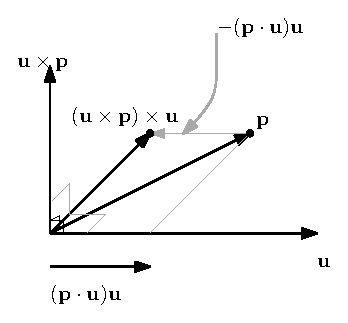
\includegraphics[width=7cm]{Math_quaternion/uxpxu.eps}
    \caption{$\mathbf u \times \mathbf p \mathbf u$와 $\mathbf p - (\mathbf p \cdot \mathbf u) \mathbf u$의 동일함에 대한 시각적 설명}
    \label{fig:quaternion:uxpxu}
\end{figure}

$\mathbf u \times \mathbf p \times \mathbf u$는 $\mathbf p - (\mathbf u \cdot \mathbf p) \mathbf u$라는 것은
그림 \ref{fig:quaternion:uxpxu}를 통해 알 수 있다. 외적의 정의에 따라 $\mathbf u \times \mathbf p \times \mathbf u$는 $\mathbf u$와 $\mathbf u \times \mathbf p$에 동시에 수직인 벡터로서 3차원 공간의 직교축을 이루게 된다. 그 크기는 $\mathbf p$를 이 축 위에 수직으로 떨어트린 위치에 의해 결정된다.
이렇게 떨어트리는 데에 필요한 길이는 $\mathbf p$와 $\mathbf u$의 내적을 통해 알 수 있고, 이를 $\mathbf u$ 축의 음의 방향으로 떨어트리면 된다.
그 결과 $\mathbf u \times \mathbf p \times \mathbf u = \mathbf p - (\mathbf p \cdot \mathbf u) \mathbf u$임을 알 수 있다.
따라서 식 \ref{eq:quaternionRotation2}는 다시 다음과 같이 바뀐다.

\begin{eqnarray}
\hat q \hat p \hat q^* =  ( 0, (\cos^2 \theta - \sin^2 \theta ) \mathbf p + 2 \sin \theta \cos \theta \mathbf u \times \mathbf p + (2 \sin^2 \theta \mathbf u \cdot \mathbf p) \mathbf u )
\label{eq:quaternionRotation3}
\end{eqnarray}



우리는 다음과 같은 사실을 알고 있다.

\begin{eqnarray}
\cos 2 \theta  & = & \cos^2 \theta - \sin^2 \theta \\ \nonumber
\sin 2 \theta & = & 2 \sin \theta \cos \theta \\ \nonumber
\end{eqnarray}

이 항등식을 적용하여 식 \ref{eq:quaternionRotation3}를 다시 정리하면 다음과 같다.

\begin{eqnarray}
\hat q \hat p \hat q^* =  ( 0, (\cos 2\theta \mathbf p + \sin 2 \theta (\mathbf u \times \mathbf p) + (2 \sin^2 \theta \mathbf u \cdot \mathbf p) \mathbf u)
\label{eq:quaternionRotation4}
\end{eqnarray}

$1=\cos^2 \theta + \sin^2 \theta$이므로 $\sin^2 \theta = 1 - \cos^2 \theta$이다.
따라서 위 식에 나타나는 $2\sin^2 \theta$는 $\sin^2 \theta + \sin^2 \theta = \sin^2 \theta + 1 - \cos^2 \theta$가 된다.
이는 곧 $1 - (\cos^2 \theta - \sin^2 \theta)$이므로 다음과 같은 식이 성립한다.

$$2 \sin^2 \theta = 1 - \cos 2 \theta$$

그러므로 식 \ref{eq:quaternionRotation4}는 다음과 같이 다시 고쳐 쓸 수 있다.

\begin{eqnarray}
\hat q \hat p \hat q^* =  ( 0, (\cos 2\theta \mathbf p + \sin 2 \theta (\mathbf u \times \mathbf p) + ((1-\cos 2 \theta) \mathbf u \cdot \mathbf p) \mathbf u)
\label{eq:quaternionRotation5}
\end{eqnarray}



\begin{figure}[h!]
  \centering
    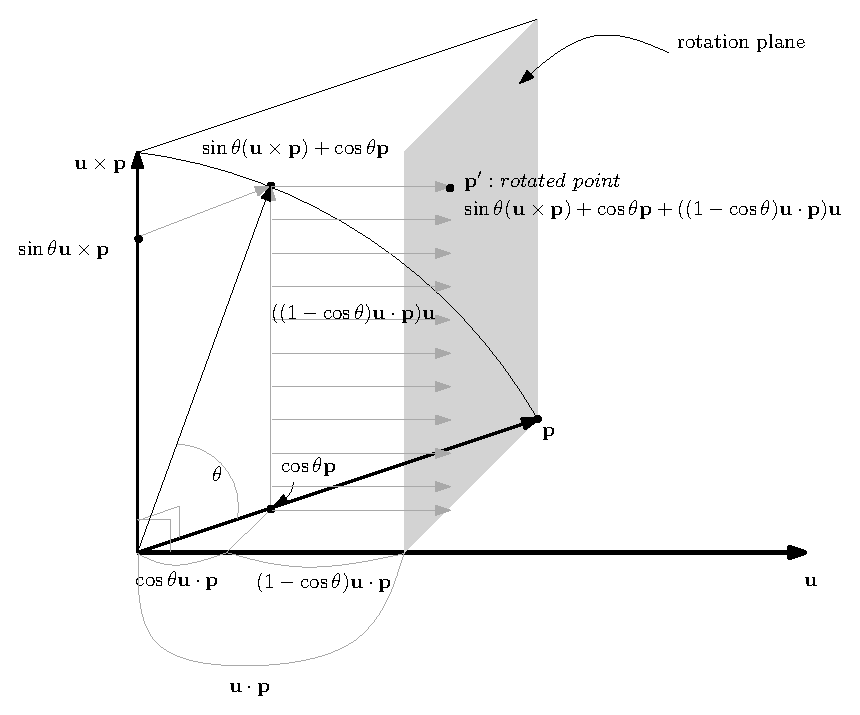
\includegraphics[width=14cm]{Math_quaternion/quaternionRotation.eps}
    \caption{임의의 $\mathbf p$를 축 $\mathbf u$를 기준으로 회전했을 때 얻게 되는 점 $\mathbf p'$}
    \label{fig:quaternion:quaternionRotation}
\end{figure}


이렇게 얻어진 결과가 회전과 어떤 관계를 갖는지를 알고 싶으면 그림 \ref{fig:quaternion:quaternionRotation}을 살펴 보자.
그림에서는 어떤 점 $\mathbf p$가 축 $\mathbf u$를 기준으로 회전하고 있다. 회전된 점들이 놓이게 되는 평면을 회전 평면이라 하면
그림의 회색 부분이 이 평면의 일부가 된다.
이점을 쉽게 찾기 위해 우선 $\mathbf p$와 $\mathbf u \times \mathbf p$를 축으로 하는 2차원 평면의 원점을 기준을 $\theta$ 만큼 회전하여 얻는 점을
먼저 살펴 보자. 이 점은 그림에서 보는 바와 같이 $\mathbf p$ 축으로의 길이는 $|\mathbf p| \cos \theta$이고,
$\mathbf u \times \mathbf p$축 방향으로의 길이는 $|\mathbf p| \sin \theta $이다.
따라서 이 점의 좌표는 $\sin \theta (\mathbf u \times \mathbf p) + \cos \theta \mathbf p$로 표현할 수 있다.
이제 이 점을 회전 평면 위로 옮기면 된다.

회전 평면위로 옮기기 위해서는 $\mathbf p$와 $\mathbf u$가 함께 지나는 평면 위로 조금 전에 구한 점을 떨어트리고 이를 회전 평면에 옮기는 데 필요한 길이를
구하면 된다. 이 길이가 $(1 - \cos \theta) \mathbf u \cdot \mathbf p$임을 쉽게 알 수 있고, 이 길이만큼 $\mathbf u$ 축으로 옮겨 놓는 벡터는
$((1-\cos \theta ) \mathbf u \cdot \mathbf p ) \mathbf u$이다.
따라서 옮겨진 점은 다음과 같다.

$$\mathbf p' = \sin \theta (\mathbf u \times \mathbf p) + \cos \theta \mathbf p +((1-\cos \theta ) \mathbf u \cdot \mathbf p ) \mathbf u$$

이 좌표는 그림 \ref{fig:quaternion:quaternionRotation}에 $\mathbf p'$로 표현된 점이다.
이 식을 식 {eq:quaternionRotation5}의 벡터 부분과 비교하면 각도 $\theta$와 $2 \theta$의 차이 있고 나머지는 모두 같다.
이것은 식 {eq:quaternionRotation5}의 사원수 곱으로 얻은 결과의 벡터 부분은 점 $\mathbf p$를 $2 \theta$ 만큼 회전시킨 것과 같다는 것이다.

이상의 결과를 이용하여 우리는 어떤 점 $\mathbf p$를 $\mathbf u$ 축을 중심으로 $\theta$ 만큼 회전하여 $\mathbf p'$를 얻고 싶을 때에 다음과 같은
연산을 수행하면 된다는 것을 알게 된다.

\begin{eqnarray}
\hat p &=& (0, \mathbf p) \\ \nonumber
\hat q &=& (\cos \frac{\theta}{2}, \sin \frac{\theta}{2} \mathbf u) \\ \nonumber
\hat p' &=& (0, \mathbf p') = \hat q \hat p \hat q^*
\end{eqnarray}
